\section{Introduction}
\label{sec:intro}

%\iffalse
%Multiple-choice questions (MCQs) are a widely used problem format 
%in Natural Language understanding tasks. 
%For example, causal reasoning task~\cite{copa2012}, story ending prediction task~\cite{roc2017,huang20story},
%argument reasoning comprehension task~\cite{arct2018} and reading comprehension task~\cite{yu2020reclor}
%are mostly in the form of MCQs which are made up of a premise and 
%two or more choices. Below is an example question taken 
%from the COPA~\cite{copa2012} dataset, which tests commonsense causal 
%reasoning~\cite{luo2016commonsense}.
%
%\begin{example}\label{ex:copa}
%An MCQ from COPA:
%\begin{description}
%\item[Premise:] The man hurt his back.
%\item[Choice 1:] He stayed in bed for several days.  \Checkmark
%\item[Choice 2:] He went to see a psychiatrist. \XSolidBrush
%\end{description}
%\end{example}
%
%Lately, some research has been devoted to explain the good performance
%of advanced neural models on such natural language~(NL) reasoning problems.
%In particular, there has been speculation that many models did not
%really ``understand'' the semantical and logical connection between
%the context and the choices, 
%but do well only due to spurious statistical features in the 
%training and test data.
%Such speculations were largely fueled by a kind of
%experiments called ``ending-only tests'' in some literatures~\cite{endingonly1,endingonly2}, 
%which we refer to as ``choice-only test'' here since our focus is 
%on multiple-choice questions.
%For example, BERT, when fine-tuned on the COPA data, can answer
%the question in \exref{ex:copa} correctly. When we remove the context from 
%the same question, and feed it to the same BERT model, it still
%gets the correct answer (Choice 1). This kind of ``choice-only'' 
%test seems to suggest that the model can make the correct prediction
%without even looking at the context of the question. 
%We call the phenomenon ``\textit{short circuit}'' in NL 
%reasoning in this paper.
%
%Despite the previous research advocating the choice-only test,
%we argue that it has an inherent flaw as a test for
%short circuit: just because the model answers correctly without
%the premise, doesn't mean the model doesn't look into the premise
%when it's given one. What we need is a test that works with questions
%that are complete with premises and choices.
%
%\begin{figure}[th!]
%\centering
%\includegraphics[width=0.6\columnwidth]{figure/end_related.eps}
%\caption{Attention map showing that BERT~\cite{devlin2018bert} 
%short-circuits on a COPA question.}
%\label{fig:att-goodex}
%\end{figure}
%
%
%Our initial attempt at a better short circuit test
%is to plot the attention map between the words in the full question 
%from the final encoder layer of the model. We show
%such a plot of \exref{ex:copa} in \figref{fig:att-goodex}.
%The diagram clearly shows that there's virtually no connection
%between the first choice and the context when the model is processing
%the full question, while the attention between the words within the
%first choice remains the same when the model processes only the choices
%without the context.
%
%Manually checking the short circuit of a model using such attention maps
%is tedious and costly. To that end, we implemented a whitebox testing
%algorithm which simulates human visualization using some thresholds. 
%The disadvantage of this is that it requires the access to the code of 
%the models and such approach only works for attention-based models.
%
%To address these challenges, we design a new operation on 
%MCQ question instances, called \textit{crossover},
%which takes two MCQs and exchange their
%choices, analogous to how chromosomes swap their segments in
%the biological reproduction. It imposes a unique challenge on models  frequently exploiting short circuit and is able to detect such behavior 
%on real tasks by constructing proxy test cases. 
%Through the lens of crossover test and  
%several other instance-level stress tests, such as named entity replacement, 
%we find evidence of short circuit in three recent powerful natural language
%reasoning models reflected by notable declines in accuracy on these tests.
%
%One straightforward way to improve model robustness is to generate more 
%training examples by the types of stress test that the model is struggling with. 
%However, many of the stress tests come with certain constraints on the choice
%construction, which limits the number of cases that can be generated
%automatically, and consequently their ability to serve as a general 
%data augmentation method. 
%Fortunately, crossover, as well as its counterpart \textit{mutation}, 
%do satisfy all the stringent requirements. 
%
%To that end, we applied crossover, mutation and back-translation~\cite{back2019} to augment
%BERT, XLNet~\cite{xlnet2019nips} and RoBERTa~\cite{roberta2019} on ROC~\cite{roc2017}, COPA, ARCT~\cite{arct2018} and RECLOR~\cite{yu2020reclor} and saw
%up to 24\% increase in accuracy on the stress tests and 10\% increase in
%the original test data.
%
%This paper makes three main contributions:
%\begin{enumerate}
%\item We propose two approaches for detecting short circuit. One is through white-box attention weight thresholding, the other is a black-box ``crossover'' test inspired by molecular biology.
%\item We experimentally verify the existence of short circuit behavior
%in three fine-tuned strong NL reasoning models. 
%\item We propose to use both crossover and mutation operations
%to augment training data that teaches the models to consider 
%contexts in questions. Our experiments confirm the validity 
%of this approach and show substantial improvement to model robustness,
%not only on the stress tests but also on the original test data.
%\end{enumerate}
%
%\fi

Multiple-choice questions (MCQs) are a widely used format for assessing Natural Language Understanding (NLU) tasks, such as causal reasoning~\cite{copa2012}, 
story ending prediction~\cite{roc2017,huang20story}, argument reasoning comprehension~\cite{arct2018}, and reading comprehension~\cite{yu2020reclor}. These tasks typically consist of a premise followed by two or more choices. For example, the COPA dataset~\cite{copa2012} tests commonsense causal reasoning~\cite{luo2016commonsense} through MCQs, as shown below.

\begin{example}\label{ex:copa}
An MCQ from COPA:
\begin{description}
\item[Premise:] The man hurt his back.
\item[Choice 1:] He stayed in bed for several days. \Checkmark
\item[Choice 2:] He went to see a psychiatrist. \XSolidBrush
\end{description}
\end{example}

Recent research has sought to explain the strong performance of advanced neural models on NLU reasoning problems. In particular, there is speculation that many models succeed not by genuinely understanding the semantic and logical connections between the context and the choices, but by exploiting spurious statistical features in the training and test data. This idea is supported by``choice-only tests'' (also known as``ending-only tests'')~\cite{endingonly1,endingonly2}, where models like BERT can correctly answer questions even when the context is removed.

In this paper, we refer to this phenomenon as``short circuit'' in Natural Language reasoning. Although choice-only tests provide some evidence for short circuit behavior, we argue that they have inherent limitations. Just because a model can answer correctly without the premise doesn't necessarily mean it doesn't consider the premise when it is provided. To address this issue, we need a test that works with complete questions, including both premises and choices.
\begin{figure}[th!]
\centering
\includegraphics[width=0.6\columnwidth]{figure/end_related.eps}
\caption{Attention map showing that BERT~\cite{devlin2018bert} 
short-circuits on a COPA question.}
\label{fig:att-goodex}
\end{figure}



Our initial attempt at a more comprehensive short circuit test involves plotting the attention map between the words in a full question from the final encoder layer of the model. We illustrate this approach using an attention map of the example from COPA (\exref{ex:copa}) in \figref{fig:att-goodex}. The diagram clearly shows that there is virtually no connection between the first choice and the context when the model processes the full question, while the attention between words within the first choice remains the same when the model processes only the choices without the context.

Manually examining the short circuit behavior of a model using attention maps is tedious and costly. To address this issue, we implement a white-box testing algorithm that simulates human visualization using threshold values. However, this approach has limitations: it requires access to the model's code and only works for attention-based models.

To overcome these challenges, we introduce a new operation called``crossover'' for MCQ question instances. Crossover exchanges the choices of two MCQs, analogous to how chromosomes swap segments during biological reproduction. This operation poses a unique challenge for models that frequently exploit short circuit behavior and can detect such behavior in real tasks by constructing proxy test cases. By examining crossover tests and other instance-level stress tests, such as named entity replacement, we find evidence of short circuit behavior in three recent, powerful NLU reasoning models, as indicated by notable declines in accuracy on these tests.

Having identified the presence of short circuit behavior, our next goal is to improve model robustness. While generating more training examples using stress tests the model struggles with might be a direct approach, many stress tests impose constraints on choice construction, limiting their effectiveness as general data augmentation methods. However, the crossover operation and its counterpart, ``mutation,'' offer a suitable solution. These operations not only allow for the detection of short circuit behavior but also serve as effective data augmentation techniques to reduce its occurrence, enhancing the overall robustness of NLU models.

To this end, we apply
crossover, mutation, and back-translation~\cite{back2019} to augment BERT, XLNet~\cite{xlnet2019nips}, and RoBERTa~\cite{roberta2019} on ROC~\cite{roc2017}, COPA, ARCT~\cite{arct2018}, and RECLOR~\cite{yu2020reclor}. Our experiments show up to a 24\% increase in accuracy on stress tests and a 10\% increase on the original test data.

This paper makes three main contributions:

\begin{enumerate}
\item We propose two approaches for detecting short circuit behavior: a white-box method based on attention weight thresholding and a black-box``crossover'' test inspired by molecular biology.
\item We experimentally verify the existence of short circuit behavior in three powerful, fine-tuned NLU reasoning models.
\item We suggest using crossover and mutation operations to augment training data, encouraging models to consider the context of questions. Our experiments confirm the effectiveness of this approach, demonstrating substantial improvements in model robustness, not only on stress tests but also on the original test data.
\end{enumerate}
